\subsection{Porcentaje de datos faltantes}
Se determinó que el conjunto de datos utilizado cuenta con 5 atributos con datos faltantes, todos con un porcentaje menor al 30\%, por lo que se puede aplicar técnicas de imputación a todos los atributos con datos faltantes. La Tabla \ref{Tab: Faltantes} muestra el detalle de los datos faltantes encontrados.

\begin{table}[htbp]
\centering
\caption{Porcentaje de datos faltantes por atributo.}
\label{Tab: Faltantes}
\begin{tabular}{|c|c|K{30mm}|K{35mm}|}
\hline 
Columna & Total de instancias & Instancias con datos faltantes & Porcentaje de datos faltantes \\ 
\hline 
sex & 40910 & 3 & 0.01\% \\ 
\hline 
age & 40910 & 0 & 0.00\% \\ 
\hline 
hypertension & 40910 & 5676 & 16.11\% \\ 
\hline 
heart\_disease & 40910 & 0 & 0.00\% \\ 
\hline 
ever\_married & 40910 & 0 & 0.00\% \\ 
\hline 
work\_type & 40910 & 5675 & 16.11\% \\ 
\hline 
Residence\_type & 40910 & 5704 & 16.20\% \\ 
\hline 
avg\_glucose\_level & 40910 & 0 & 0.00\% \\ 
\hline 
bmi & 40910 & 5720 & 16.25\% \\ 
\hline 
smoking\_status & 40910 & 0 & 0.00\% \\ 
\hline 
stroke & 40910 & 0 & 0.00\% \\ 
\hline 
\end{tabular} 
\end{table}

\subsection{Histogramas con datos originales}
Observando los histogramas de todas las columnas del conjunto de datos (mostrados en la Figura \ref{Fig: HistOR} podemos observar lo siguiente de los atributos con datos faltantes.

\begin{itemize}
	\item \textbf{sex, hypertension, Residence\_type}
		\begin{itemize}
			\item Los datos faltantes son categóricos.
			\item Los datos faltantes sólo pueden tomar los valores 0 o 1.
		\end{itemize}
	\item \textbf{work\_type}
		\begin{itemize}
			\item Los datos faltantes son categóricos.
			\item Los datos faltantes sólo pueden tomar los valores 1, 2, 3, o 4.
		\end{itemize}
	\item \textbf{bmi}
		\begin{itemize}
			\item Los datos faltantes son continuos.
		\end{itemize}	
\end{itemize}

\begin{figure}[htbp]
	\centering
	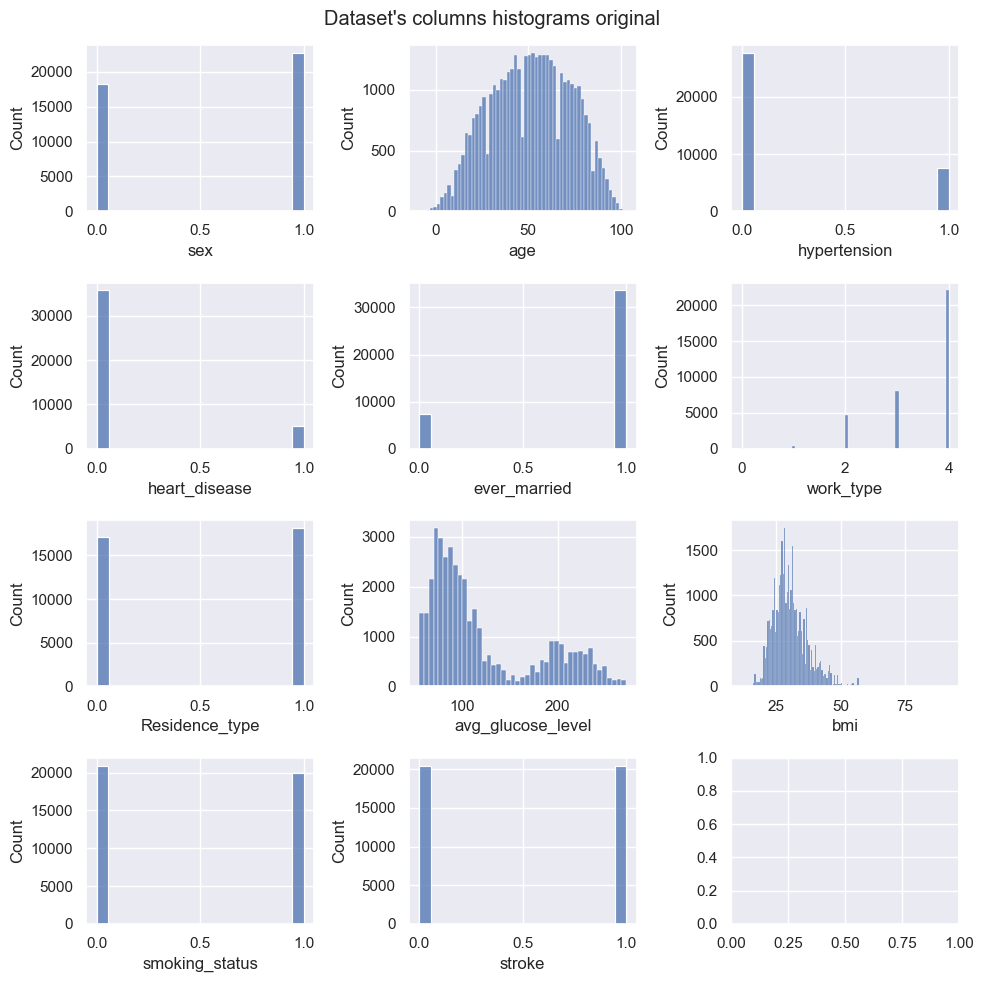
\includegraphics[width=0.9\textwidth]{dataset_histogram_original}
	\caption{Histogramas de datos originales.}
	\label{Fig: HistOR}
\end{figure}

\newpage
\subsection{Mapa de calor de correlación}
Al analizar el mapa de calor de correlación (Figura \ref{Fig: HeatMap}) se puede observar lo siguiente:

\begin{itemize}
	\item Los atributos \emph{work\_type} y \emph{Residence\_type} presentan índices de correlación cercanos a cero, por lo que la \emph{imputación aleatoria} podría aplicarse correctamente.
	
	\item El atributo \emph{hypertension} consigue su mayor índice de correlación con la variable objetivo (\emph{stroke}), por lo que una imputación por \emph{moda de clases} es una elección apropiada.

	\item El atributo \emph{bmi} consigue su mayor índice de correlación con el atributo \emph{avg\_glucose\_level}, y dado que ambos son atributos de tipo continuo la \emph{imputación por correlación} presenta una alternativa tentadora.
\end{itemize}

\begin{figure}[htbp]
	\centering
	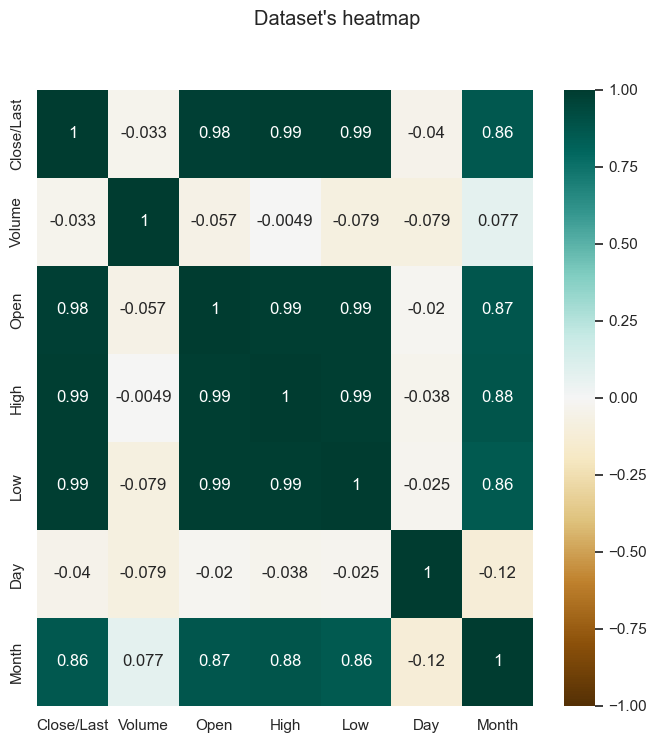
\includegraphics[width=0.65\textwidth]{dataset_heatmap}
	\caption{Mapa de calor de correlación entre columnas del conjunto de datos.}
	\label{Fig: HeatMap}
\end{figure}

\subsection{Histogramas con datos imputados}
Prestando especial atención a los atributos que se sometieron a métodos de imputación, se puede observar que el procedimiento no ha cambiado la forma de la distribución de los datos, lo cuál es un indicador de una correcta implementación de los métodos de imputación.

\begin{figure}[htbp]
	\centering
	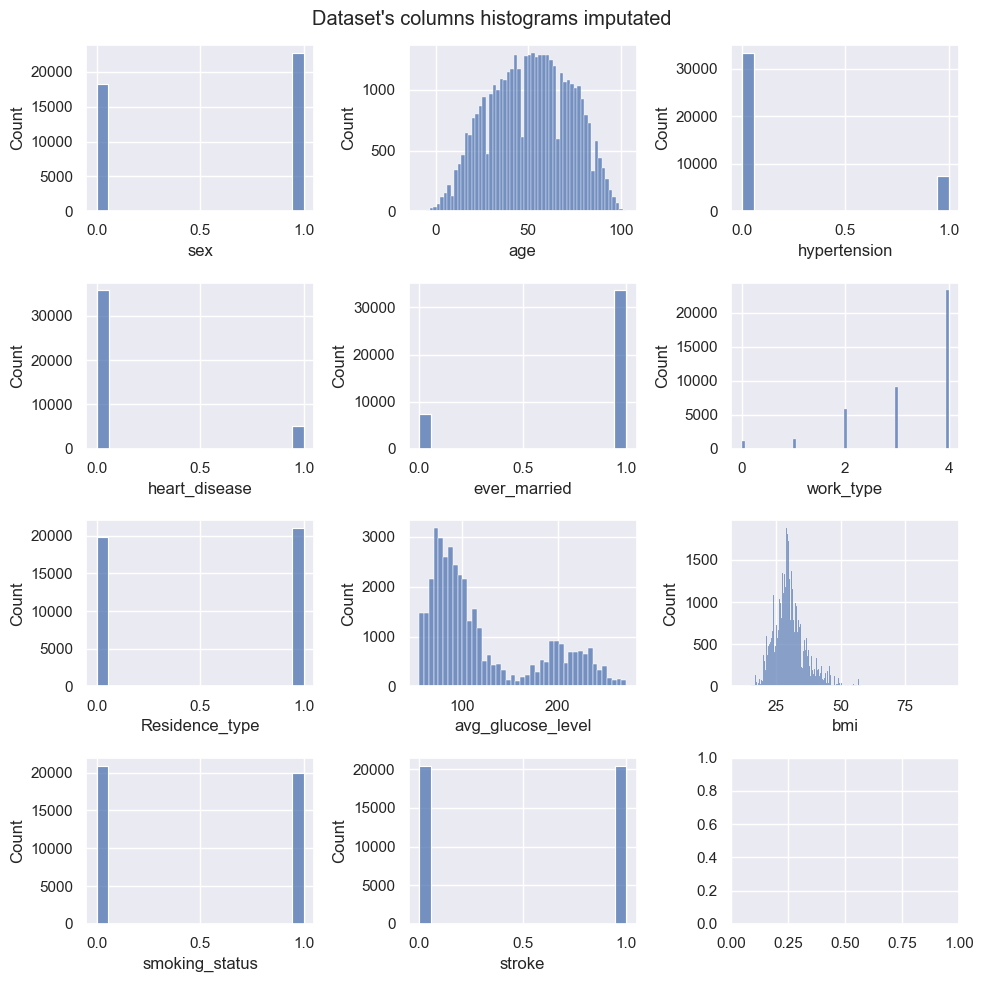
\includegraphics[width=0.9\textwidth]{dataset_histogram_imputated}
	\caption{Histogramas de datos originales con datos imputados.}
	\label{Fig: HistIM}
\end{figure}
